\documentclass[11pt]{article}

\usepackage[margin=1in]{geometry}
\usepackage[T1]{fontenc}
\usepackage[utf8]{inputenc}
\usepackage{lmodern}
\usepackage{microtype}
\usepackage{graphicx}
\usepackage{float}
\usepackage{setspace}
\usepackage{titlesec}
\usepackage{xcolor}
\usepackage{enumitem}
\usepackage{caption}
\usepackage{subcaption}
\usepackage[round,authoryear]{natbib}
\usepackage[colorlinks=true,linkcolor=blue!50!black,citecolor=blue!50!black,urlcolor=blue!50!black]{hyperref}

\graphicspath{{images/}}
\setstretch{1.1}
\setlength{\parindent}{0pt}
\setlength{\parskip}{0.7em}
\setlist[itemize]{leftmargin=1.5em}
\captionsetup{font=small,labelfont=bf}

\titleformat{\section}{\large\bfseries}{\thesection.}{0.5em}{}
\titleformat{\subsection}{\normalsize\bfseries}{\thesubsection.}{0.5em}{}
\titlespacing*{\section}{0pt}{1.2em}{0.4em}
\titlespacing*{\subsection}{0pt}{0.9em}{0.3em}

\begin{document}

\begin{center}
    {\LARGE\bfseries BNPL as a Dark Pattern and an Unintended Consequence\par}
    \vspace{0.35em}
    {\large LIS 470 Assignment 9\par}
    \vspace{0.75em}
    {\normalsize Alejandro De La Torre\par}
    {\normalsize April 20, 2026\par}
\end{center}

\vspace{1em}

\section{Introduction}

Here, we reflect on a recent online shopping experience I had, purchasing Allen Edmonds dress shoes, to analyze both parts of Assignment 9. The same interface works as a \textit{dark pattern} at the level of the individual transaction and as an \textit{unintended consequence} at the level of broader social impact. My original goal was simple: pick a size, add the shoes to my cart, and complete a normal checkout. I did not open the site intending to finance the purchase. Instead, the site repeatedly foregrounded buy now, pay later (BNPL) options such as Klarna and Afterpay across the entire shopping flow.

That repetition matters. BNPL is not presented as a neutral payment alternative that appears once at the end. It is treated as a privileged, low-friction path. The interface repeatedly reframes a \$269 purchase as ``as low as 4 payments of \$67.25,'' places quick-checkout BNPL buttons in prominent positions, and then routes the user into a lightweight Klarna flow that asks only for a phone number before continuing. The result is a shopping experience that makes debt feel ordinary, convenient, and almost invisible.

\section{Dark Pattern: Steering the User Toward Installment Credit}

The dark pattern in this case is not a single deceptive pop-up. It is a sequence of interface choices that steadily increase the salience of installment credit. Figure~\ref{fig:product-bnpl} shows the product page, where the full price appears directly above a BNPL breakdown placed under the main \texttt{Add to Cart} button. That placement matters because it inserts financing into the decision before the user has even committed to the item. Rather than asking only ``Do I want these shoes for \$269?'', the interface also asks, more subtly, ``Would this feel easier as four smaller payments?''

\begin{figure}[H]
    \centering
    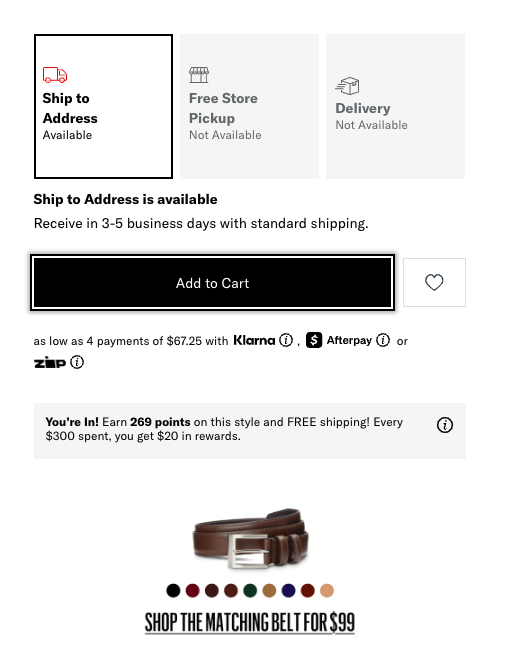
\includegraphics[width=0.42\textwidth]{buy-now-pay-later.png}
    \caption{On the product page, BNPL is surfaced immediately below the main \texttt{Add to Cart} button and reframes the purchase as four smaller payments rather than one full price.}
    \label{fig:product-bnpl}
\end{figure}

The repeated surfacing becomes even clearer after the item is added to the cart. In Figure~\ref{fig:cart-checkout}, the cart page offers a standard black \texttt{Checkout} button, but then immediately presents a second cluster of ``check out quickly with'' options, including Klarna and Afterpay. The same screen repeats the installment framing again in the order summary. The checkout page continues the pattern by placing quick-checkout buttons above the ordinary contact and shipping forms. In other words, the site does not merely allow BNPL. It repeatedly positions BNPL as the faster and more streamlined path.

\begin{figure}[H]
    \centering
    \begin{subfigure}[t]{0.48\textwidth}
        \centering
        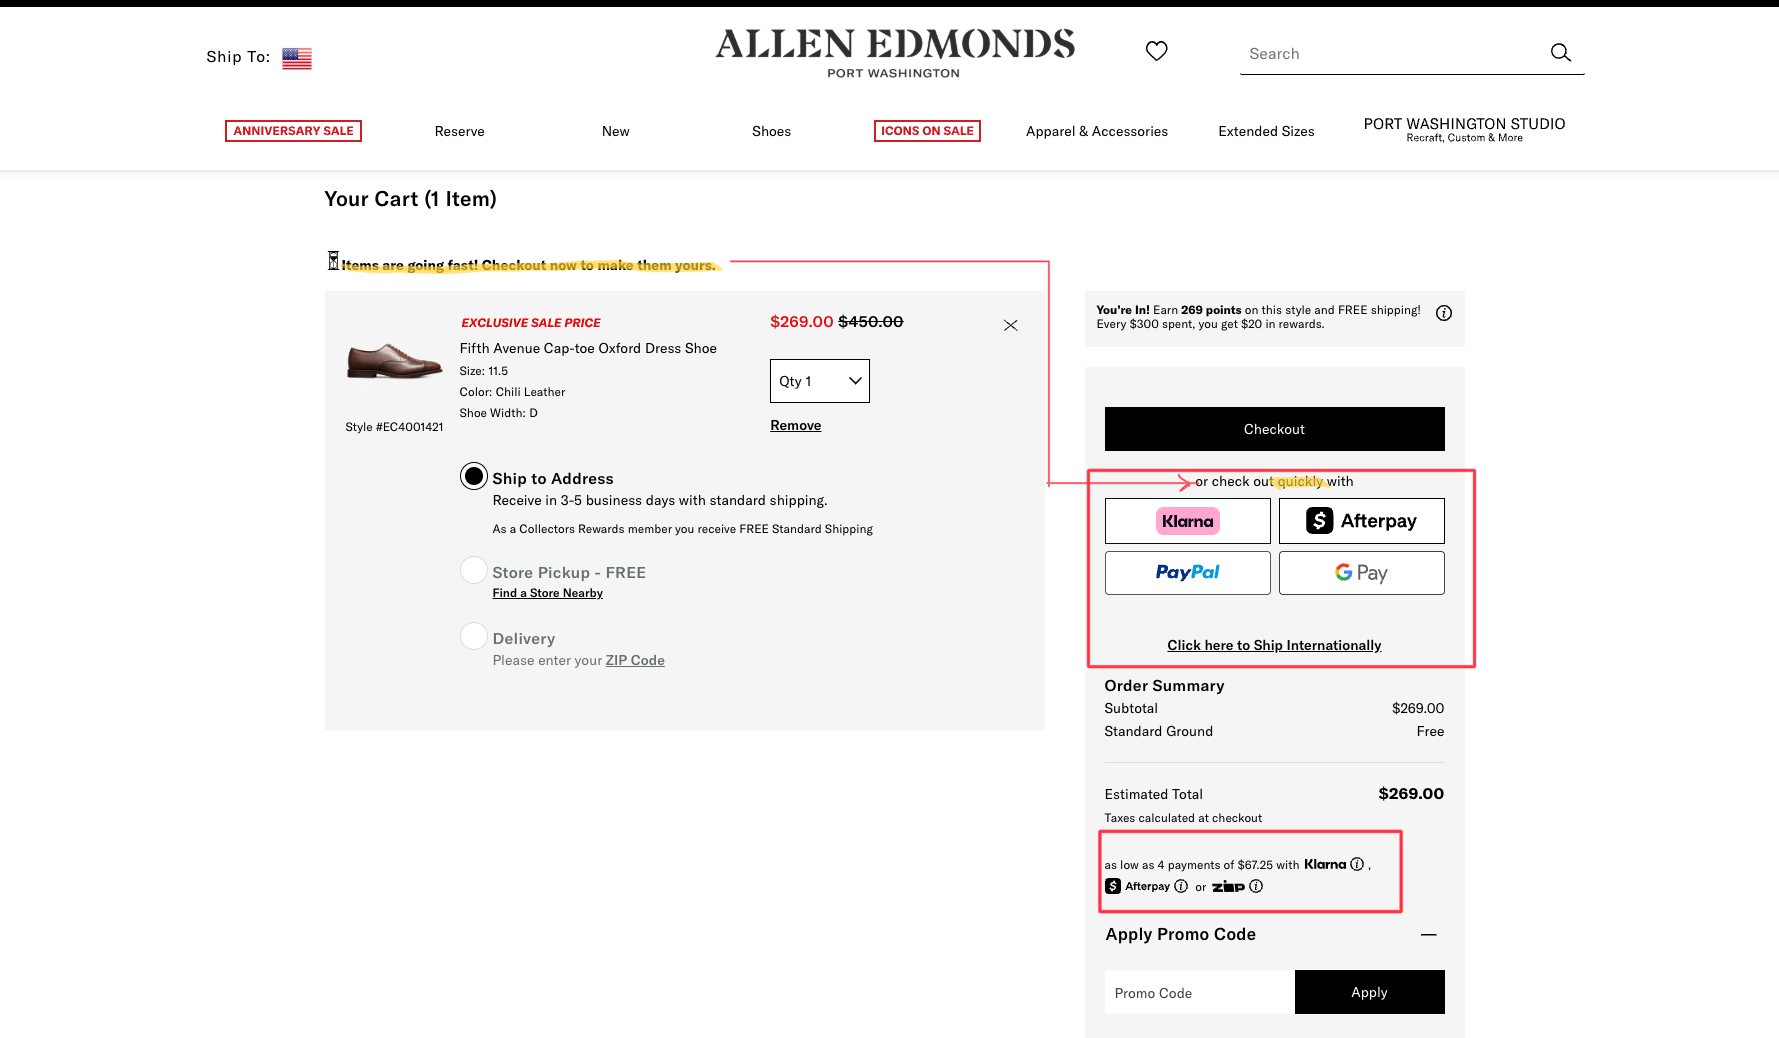
\includegraphics[width=\linewidth]{cart-screen.png}
        \caption{The cart screen presents BNPL twice: first as quick-checkout buttons, and again as installment language next to the order total.}
    \end{subfigure}
    \hfill
    \begin{subfigure}[t]{0.48\textwidth}
        \centering
        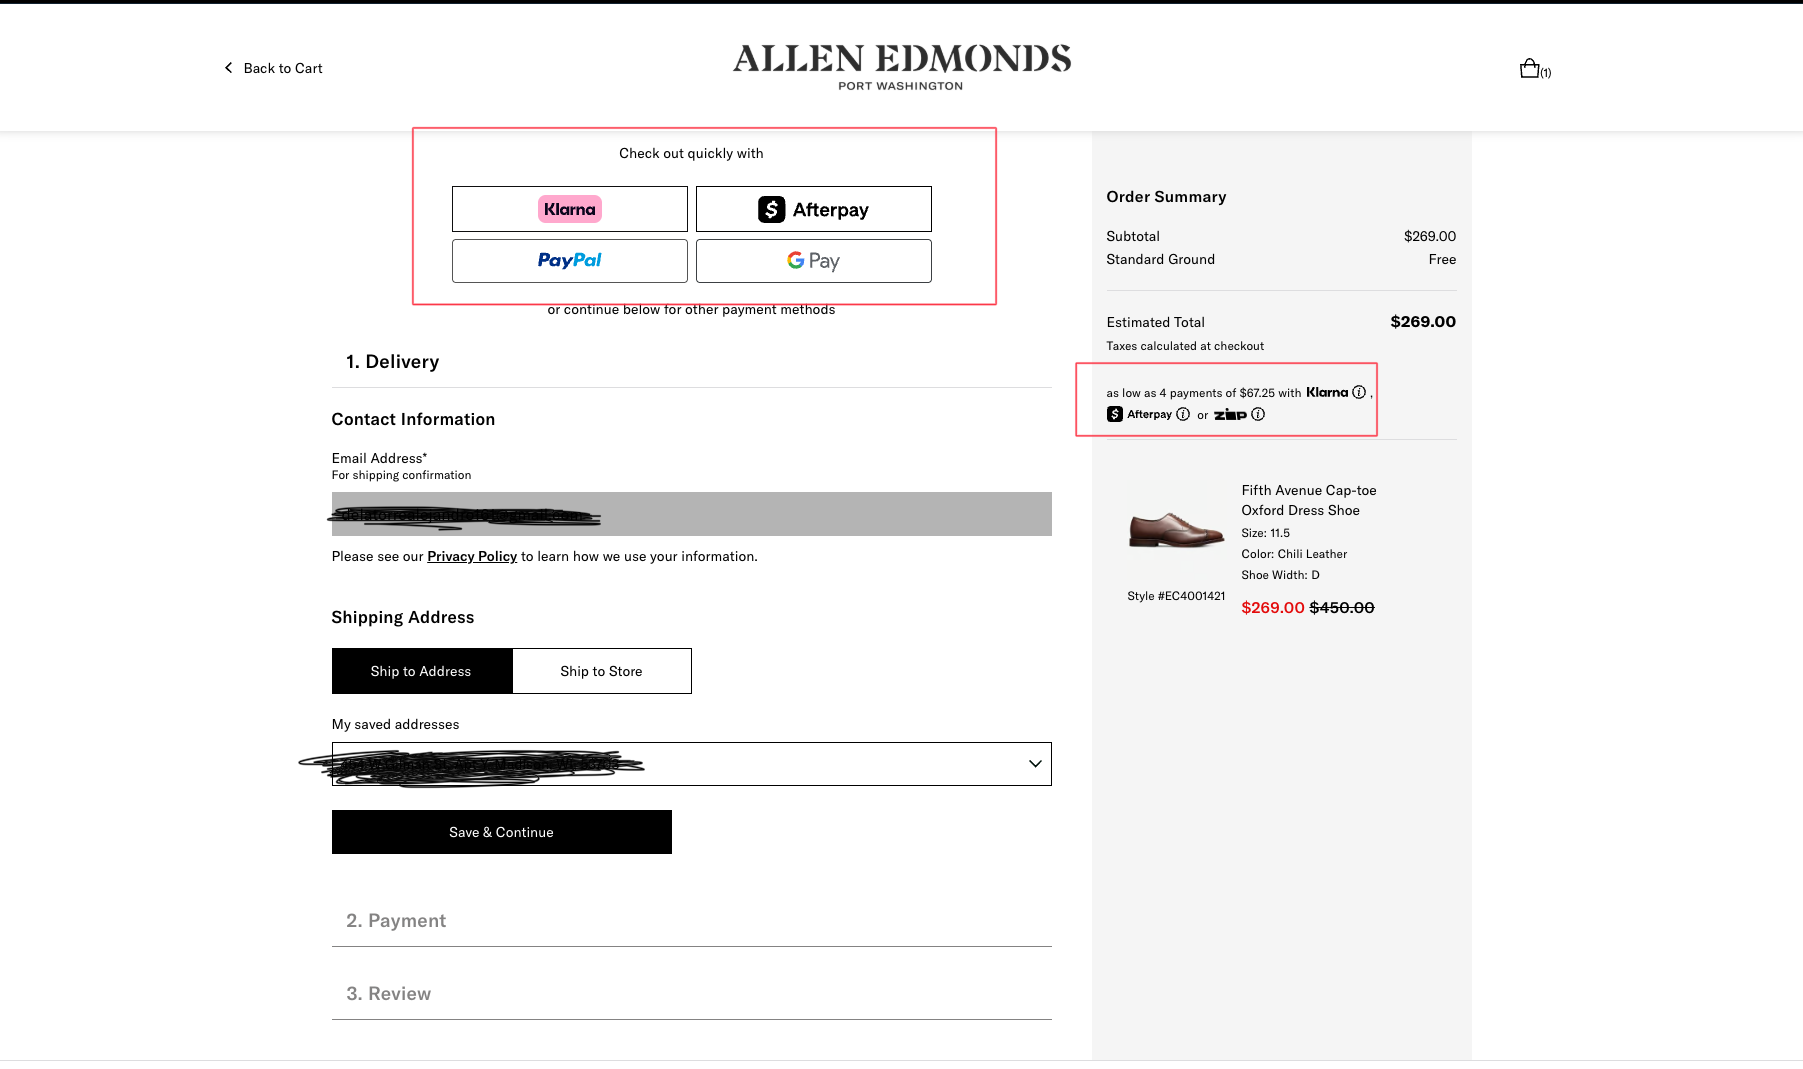
\includegraphics[width=\linewidth]{checkout.png}
        \caption{The checkout screen repeats the same quick-pay options before the standard form fields, giving installment credit more visual priority than ordinary checkout.}
    \end{subfigure}
    \caption{BNPL is repeatedly foregrounded throughout the shopping flow rather than being presented once as a neutral payment method.}
    \label{fig:cart-checkout}
\end{figure}

This is where the user's intended action and the likely unintended action diverge. The user intended to complete a standard purchase using a traditional payment method, but the interface makes it likely that they instead select a BNPL option they did not initially plan to use. My intended action was to buy a pair of shoes, not to open a short-term credit flow simply because it looked faster or easier. That is a form of interface interference: the design privileges one option through prominence and convenience rather than through explicit argument. It also creates asymmetric friction. Standard checkout requires contact information, shipping details, billing details, and card entry, while the BNPL route is signaled as lighter-weight and more immediate.

Figure~\ref{fig:klarna} makes that asymmetry especially visible. After selecting Klarna, the user is moved into a modal that asks for only a phone number and emphasizes reassuring messages such as ``no credit impact'' and ``buyer protection always included.'' The ordinary checkout path still exists, but it is now the slower-looking option. A user who did not arrive intending to borrow can still drift into borrowing because the interface has arranged the decision so that financing appears to be the easiest path through the purchase.

\begin{figure}[H]
    \centering
    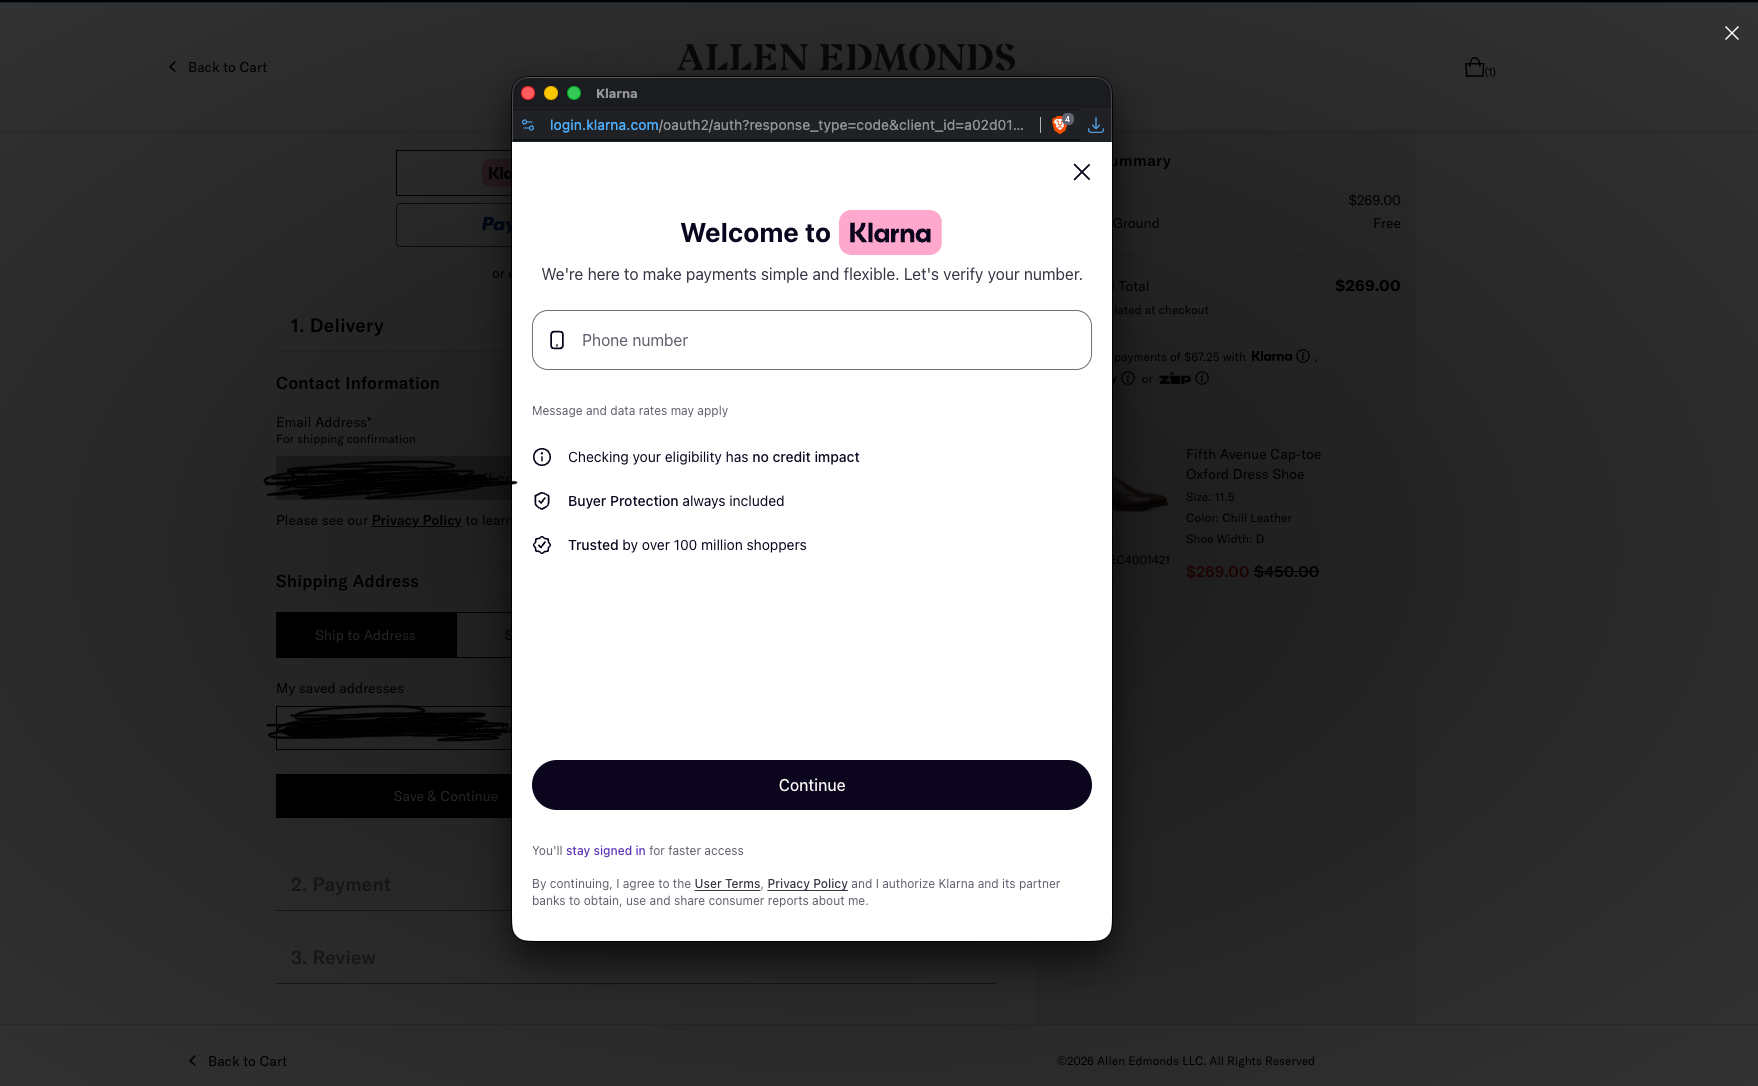
\includegraphics[width=0.88\textwidth]{klarna.png}
    \caption{Selecting Klarna opens a lightweight verification flow centered on a phone number, reinforcing the sense that BNPL is the lowest-friction way to finish the purchase.}
    \label{fig:klarna}
\end{figure}

If this interface were redesigned to make unintended credit use less likely, several changes would help. First, the full price should remain the primary frame, while installment language should be clearly labeled as credit and moved to the final payment step. Second, BNPL should not be repeated at every stage of the flow. Third, the site should avoid rewarding the credit option with noticeably less friction than the standard checkout path. Convenience is not neutral when it is distributed unevenly.

\section{Unintended Consequence: Normalizing Debt-Financed Consumption}

While the previous section shows how BNPL functions as a dark pattern at the interaction level, the same design logic scales into a broader unintended consequence at the societal level.

The intended purpose of BNPL design is easy to understand: it offers payment flexibility, reduces checkout friction, and probably increases conversion rates. The unintended consequence is broader and more troubling. By breaking a price into smaller units, repeating that framing across screens, and making installment checkout feel unusually seamless, the interface can normalize debt-financed consumption and weaken awareness of the total cost.

That concern is consistent with the literature. Mitchell argues that BNPL products often fit awkwardly around traditional consumer-credit regulation, leaving borrowers with fewer protections and less transparent disclosures than they might expect from more familiar lending products \citep{mitchellBuyNowPay2023}. O'Brien, Ramsay, and Ali likewise describe BNPL as easily accessible credit that can produce real hardship, especially for lower-income users who are already managing tight budgets \citep{obrienInnovationDisruptionConsumer2024}. What the screenshots add is a design-level explanation for why that harm is plausible: the interface does not simply offer credit, it actively reorganizes attention around the installment amount instead of the full obligation.

This is also where behavioral economics becomes relevant. Research on high-cost borrowing shows that many borrowers are present-focused and recognize a mismatch between short-term convenience and their longer-term preferences \citep{allcottNBERWORKINGPAPER}. In adjacent work on predatory lending, Hill and Kozup describe how aggressive credit practices can be wrapped in an inviting, seemingly helpful presentation that obscures downstream risks \citep{hillConsumerExperiencesPredatory2007}. BNPL interfaces are visually cleaner and less overtly coercive than classic predatory-lending examples, but the ethical concern is similar: design can make borrowing feel lighter than it really is.

What makes this an unintended consequence, rather than just a bad individual decision, is scale. A single shopper may only encounter one installment prompt. Across millions of transactions, however, repeated prompts and low-friction credit pathways can shift expectations about how ordinary consumption should happen. A purchase no longer needs to be affordable in full right now; it only needs to feel manageable when sliced into four pieces. That shift obscures full-cost awareness and can make debt feel like default shopping infrastructure rather than a meaningful financial commitment.

To reduce that unintended consequence, the design should keep the full price visually primary and label BNPL explicitly as a credit product rather than just another convenience feature. BNPL prompts should appear only at the final payment step instead of being repeated across the shopping flow, and the interface should stop centering the installment amount as the main frame for evaluating the purchase. Those changes would preserve payment flexibility while making the financial tradeoff clearer and less likely to become normalized.

\section{Design Lessons for Our Grocery Planning App}

This analysis matters for our group grocery-planning project because our app is supposed to support planning, budgeting, and coordination, not just reduce clicks. It would be easy to borrow the wrong lessons from the Allen Edmonds flow. A conversion-driven mindset might suggest that the ``best'' interface is simply the one that makes every action instant and frictionless. But for a budgeting app, that can become manipulative very quickly.

Our app should therefore preserve budget salience instead of fragmenting or hiding cost. The full grocery total should remain visible, and each roommate's share should stay legible whenever items are added, removed, or reassigned. We also should not make it too easy for one person to shift financial responsibility onto roommates without confirmation. If our interface allowed a user to offload costs with one quick tap, it would mirror the same ethical problem as BNPL: moving a burden somewhere else while making the transfer feel trivial. In a shared household setting, that kind of convenience could create confusion, resentment, or unfairness.

This is where ``ethical friction'' becomes useful. Good design is not whatever removes the most effort. Mature design removes unnecessary friction while preserving the friction that protects users' long-term interests. In our grocery app, that means confirming cost-sharing changes, showing clear before-and-after totals, and keeping budget tradeoffs visible instead of burying them under convenience features. Ease of use still matters, but it has to be aligned with transparency, consent, and fair coordination.

\section{Conclusion}

The Allen Edmonds checkout flow shows how BNPL can function as both a dark pattern and an unintended consequence. At the interaction level, the site nudges users toward installment credit by repeatedly foregrounding BNPL and giving it a lower-friction path than ordinary payment. At the societal level, the same design logic can normalize debt-financed consumption and make the full cost of a purchase less psychologically salient. A better design would keep the total price primary, present credit as credit, and avoid rewarding the indebted path with special convenience. Those same principles should guide our grocery-planning app if we want usability to support users' long-term interests instead of quietly working against them.
\newpage
\bibliographystyle{plainnat}
\bibliography{references/a9}

\end{document}
